\subsubsection{Subsystem Overview}
 The PLB manages the hardware-accelerated ML application, performs additional pre/post-processing on ML data (if required by the ML application), and communicates with the platform management board.

A decomposition of the system is seen in Figure \ref{pcdiag}.

Of note is the distinction between the two portions present in the PLB: the Hard Processor System (HPS) and the FPGA. The Hard Processor System is a non-customizable CPU and is used for generic tasks such as managing I/O via the Ethernet port and processing non-acceleratable ML tasks. The FPGA provides the system's \textit{programmable circuity} -- performing the requisite hardware acceleration needed for ML tasks. The two systems co-reside on the same chip, and are interfaced via an internal bus.

\subsubsection{Device Selection}
The selected programmable logic board is the \textit{ZedBoard SoC Development Board} (pictured in Figure \ref{zedboard}), manufactured by Digilent. 

\begin{figure}
\centering
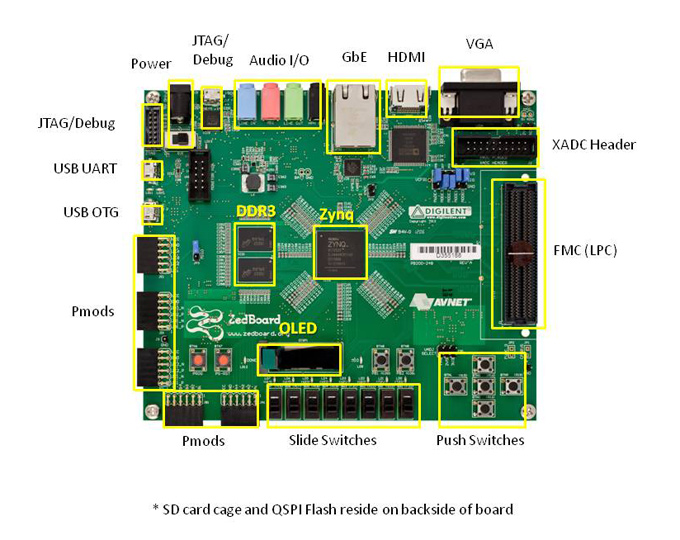
\includegraphics[width=12.5cm]{img/zedboard_functional_overview.jpg}
\caption{Layout of Connectors and Main ICs on ZedBoard\cite{zedboard}}
\label{zedboard}
\end{figure}

The system specifications are as follows\cite{zedboard}:
\begin{itemize}
\item Xilinx Zynq-7000 AP SoC XC7Z020-CLG484
\item Dual-core ARM Cortex-A9 (\textit{HPS})
\item 512 MB DDR3 Random Access Memory
\item 256 MB Quad-SPI Flash Memory
\item 10/100/1000 Ethernet 
\item USB OTG 2.0 and USB-UART 
\item PS \& PL I/O expansion (FMC, Pmod, XADC)
\end{itemize}

The selection of this particular programmable logic board was mainly motivated by cost. The client was able to provide several ZedBoard units free-of-charge, stemming from donations through the Xilinx University Program. While this board has a fairly small number of logical cells (85,000 LCs) compared to other programmable logic boards on the market, especially those which target video applications, the project's budget does not allow for the purchase of more performant boards without significant sacrifices to the multirotor assembly. The number of logical cells on the ZedBoard is sufficient to comply with the minimum LC constraint (\textbf{C.EX.1}).

Examples of other boards examined for this project include the Nexys Artix 7 FPGA (200,000 LCs, US\$479)\cite{nexys} and the Microsemi PolarFire Video/Imaging FPGA (300,000 LCs, CAN\$1500)\cite{microsemi}. Use of the Terasic DE1-SoC (another board available free-of-charge from the client, 85,000 LCs) was also considered, but was ultimately not selected due to its poorer I/O selection (no FSC/HDMI connections, which could be used by the client to expand the system) and more complicated development toolchain.

\subsubsection{Data Flow}
The overall data flow managed by the PLB is as follows:
\begin{enumerate}
\item Video/ML input data is acquired by the HPS (ARM core) via the Ethernet port (from the PMB)
\item The HPS, managing the machine learning, splits the input data into ML \textit{subtasks} (such as matrix-matrix multiply, pooling, etc)
\item Where hardware acceleration of a particular ML subtask is possible, the requisite data is sent from the HPS to the FPGA via a bi-directional AXI interface
\item The ML IP block on the FPGA receives subtasks to be accelerated via the AXI bus, performs the requisite processing, and sends the results to the HPS (on the same bus)
\item When all ML subtasks are complete, the HPS sends the results of the task back to the PMB (Raspberry Pi) via the Ethernet port
\end{enumerate}

\subsubsection{ML Hardware Accelerator Implementation}
To facilitate the hardware acceleration of ML subtasks, a customized version of the open-source MARLANN (\textit{Multiply-Accumulate and Rectified-Linear Accelerator for Neural Networks}) module will initially be used\cite{marlann}. As the client intends to replace this module with a custom-designed solution stemming from their research, however, it is only intended as a placeholder.

MARLANN is capable of performing 8-bit fixed point signed integer arithmetic, matrix multiplication, and max-pooling. After evaluating other open-source FPGA-based accelerators, MARLANN was selected due to its low FPGA area overhead (approx. 5,000 LCs), efficient pipelined architecture, and comprehensive documentation. The use of a pre-designed accelerator also allows the designers to quickly deploy simple ML models without the considerable hardware design overhead implicit in a full-custom solution.
